\section{Versionsverwaltung} \label{sec:tech-Versionsverwaltung}
Eine Versionsverwaltung ist ein System der Softwareentwicklung zur Versionierung und Kontrolle des gemeinsamen Zugriff's auf Quelltexte. Mit Hilfe einer solchen Software werden laufende �nderungen an Quelltexten oder �hnlichen Dateien erfasst und in einem Archiv mit Zeitstempel und Benutzerkennung erfasst. Ein Archiv, auch Repository genannt, ist dabei meist einen Datenbank oder ein systemabh�ngiges Dateiformat. Mit Hilfe einer Versionsverwaltung k�nnen mehrere Benutzer (Entwickler) einem einem Projekt, sogar an einer Datei gleichzeitig arbeiten. Ohne des Einsatz einer Versionsverwaltung ist es sehr schwierig in einem Team eine Software zu entwickeln. Jeder Entwickler muss immer den aktuellen Stand der Quelltexte besitzen und m�sste sich mit den anderen Entwickler absprechen, welche Dateien von wem bearbeitet werden, eine gleichzeitige Bearbeitung einer Datei w�re nur mit gro�em Aufwand m�glich, wie in \vref{fig:vv-personen} beispielhaft zu sehen ist. Weiterhin ist es in Fehlerf�llen schwierig auf �ltere Projektst�nde zur�ckzugreifen. Da in der heutigen zeit viele Projekte global, von mehreren Entwicklern weltweit, unter Zeitdruck entwickelt werden, ist der Einsatz einer Versionsverwaltung zwingend notwendig. Eine Versionsverwaltung �bernimmt dabei folgende Aufgaben:
\begin{itemize}[itemsep=.5cm]
	\item fr�here Versionen reproduzierbar
	\item kontinuierliche Generationsfolge sicherstellen
	\item Platzsparende Speicherung
	\item Schutz vor unberechtigtem Zugriff
	\item Kostenreduzierung
\end{itemize}
\begin{figure}[tbp]
	\centering
	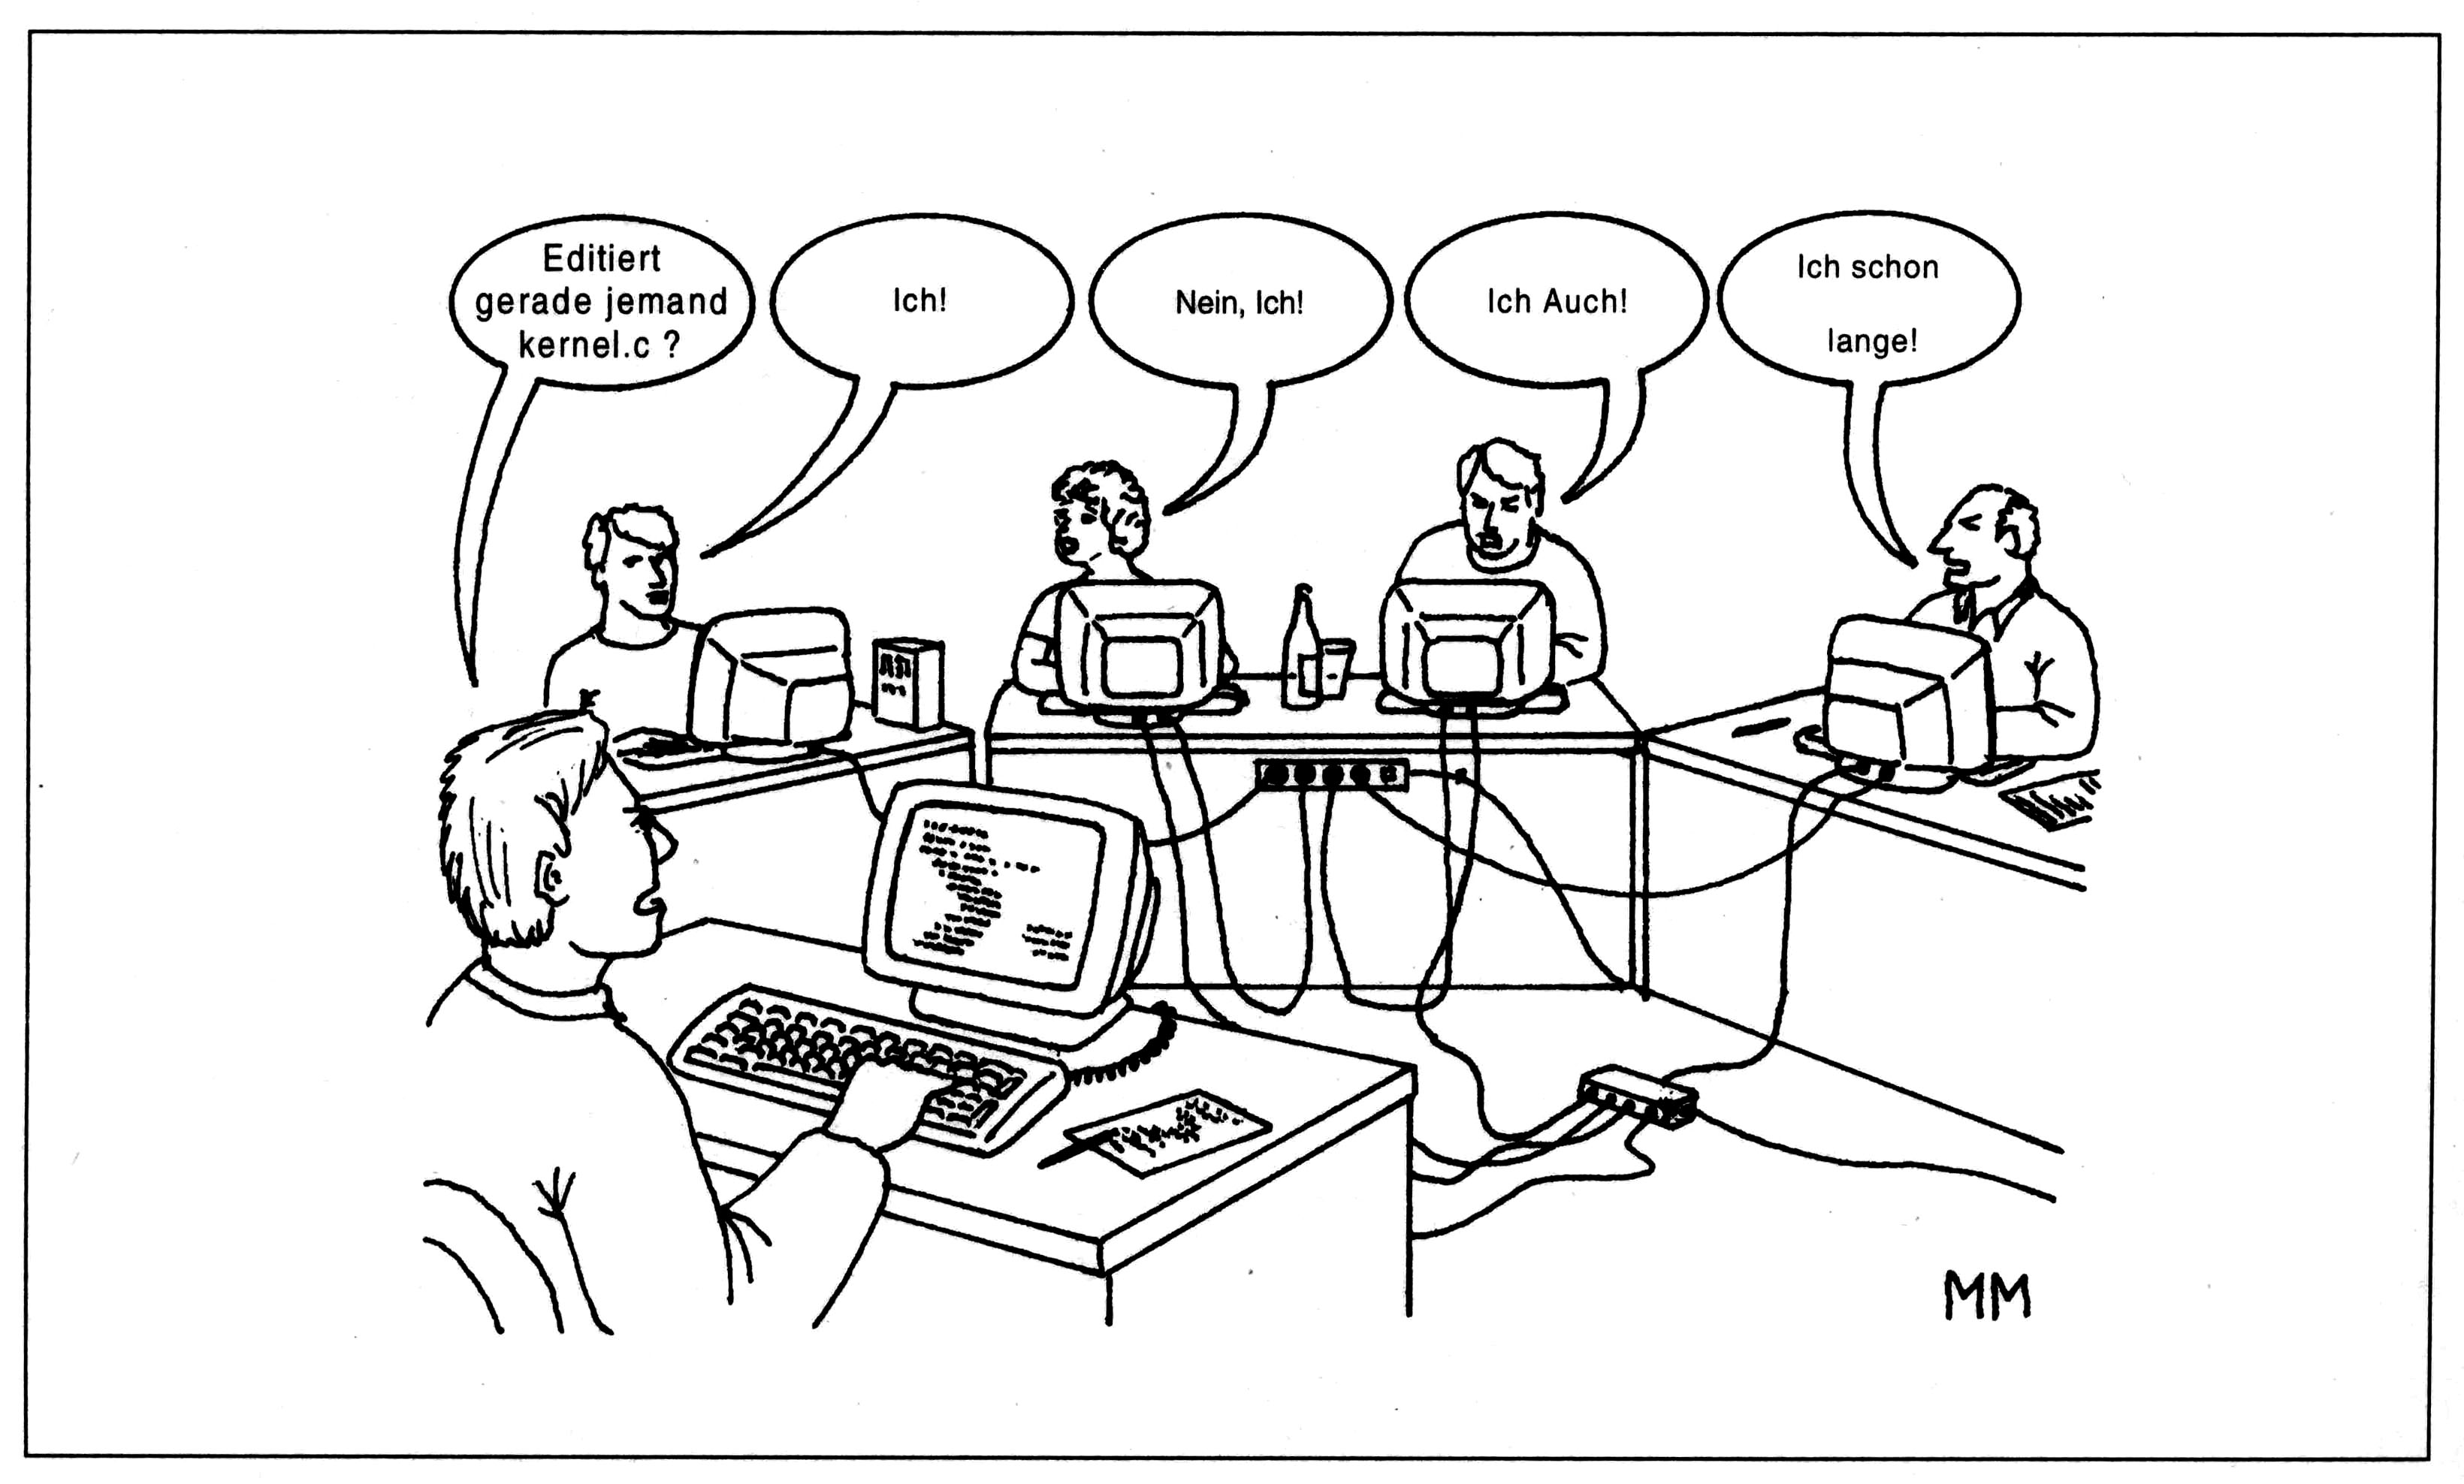
\includegraphics[scale=0.45]{images/vv-personen.jpg}
	\caption{Softwareentwicklungs-Praxis \citep[Bild 2.1]{Herold1995}}
	\label{fig:vv-personen}
\end{figure}
Jeder Entwickler muss eine \emph{Arbeitskopie} des Projektes vom Repository anfordern. Dieser Vorgang wird als \emph{"`Checking out"'} bezeichnet und einmalig am Anfang erfolgen. Danach aktualisiert er seine Arbeitskopie auf den aktuellsten Stand des Repository. Bei der Speicherung (\emph{"`Commit"'}) der neuen Zus�nde der Quelltexte in dem Repository werden den einzelnen Dateien oder dem aktuellen Projektstand eine aufsteigende Nummer vergeben. Somit wei� der Entwickler, dass der sich gerade in \emph{Revision} 13.2 befindet. Da jede Revision in dem Repository gespeichert wird, ist es dem Entwickler m�glich, auf �ltere Revisionen zur�ckzugreifen und somit �ltere Dateien betrachten. Dies ist bspw. notwendig um �nderungen nach zu vollziehen bei eventuellen aktuellen Fehlern. Weiterhin m�ssen wichtige z.Z. nicht nben�tigte Teile des Quelltextes nicht auskommentiert werden, sondern k�nnen gel�scht werden. Somit k�nnen \emph{fr�here Versionen reproduziert} werden. Durch die automatische Vergabe der Revisionsnummern, wird weiterhin die \emph{kontinuerliche Generationsfolge} sichergestellt. Der Entwickler ist gezwungen vor dem Speichern seiner Quelltexte in dem Repository, die aktuelle Revision aus dem Repository zu laden. Denn nur dadurch wird sichergestellt, dass nach der Speicherung der Revision 13.2 die Revision 13.3 folgt. M�chten bspw. zwei Entwickler eine Datei editieren und letztendlich zum Repository hinzuf�gen, m�ssen beide vor dem Speichern die aktuellste Version laden. \Vref{fig:kontinuerlicheEntwicklung} veranschaulicht den dargestellten Sachverhalt. Dabei m�chten sowohl \emph{EntwicklerA} als auch \emph{EntwicklerB} eine Datei \emph{QuellcodeA.txt} zu bearbeiten. Zum gleichen Zeitpunkt aktualisieren beide ihre lokale Arbeitskopie zur aktuellen Revision \emph{13.2} und beginnen die Datei zu ver�ndern. EntwicklerB ist nach einer kurzen Zeit mit seinen �nderungen fertig und m�chte diese im Repository speichern. Diese Aktion wird erfolgreich vom Versionsverwaltungsserver quittiert, indem die Revision 13.3 vergeben wird und somit die aktuelle Revision der Datei \emph{QuellcodeA.txt} ist. EntwicklerB ist mit seiner Arbeit an dieser Datei fertig. Nach einer Weile m�chte EntwicklerA seine �nderungen im Repository speichern und versucht dies. Der Versionsverwaltungsserver wird dem EntwicklerA mitteilen, dass seine lokale Kopie mit der Versionsnummer 13.2 nicht mehr die aktuellste ist und zwingt den EntwicklerA zuerst die aktuelle Revision der zu speichernden Datei zu laden. Nachdem der EntwicklerA dies getan hat, muss er eventuelle Konflikte zwischen beiden Dateien beheben und kann danach die Datei im Repository mit der Revisionnummer 13.4 speichern.
\begin{figure}[tbp]
	\centering
	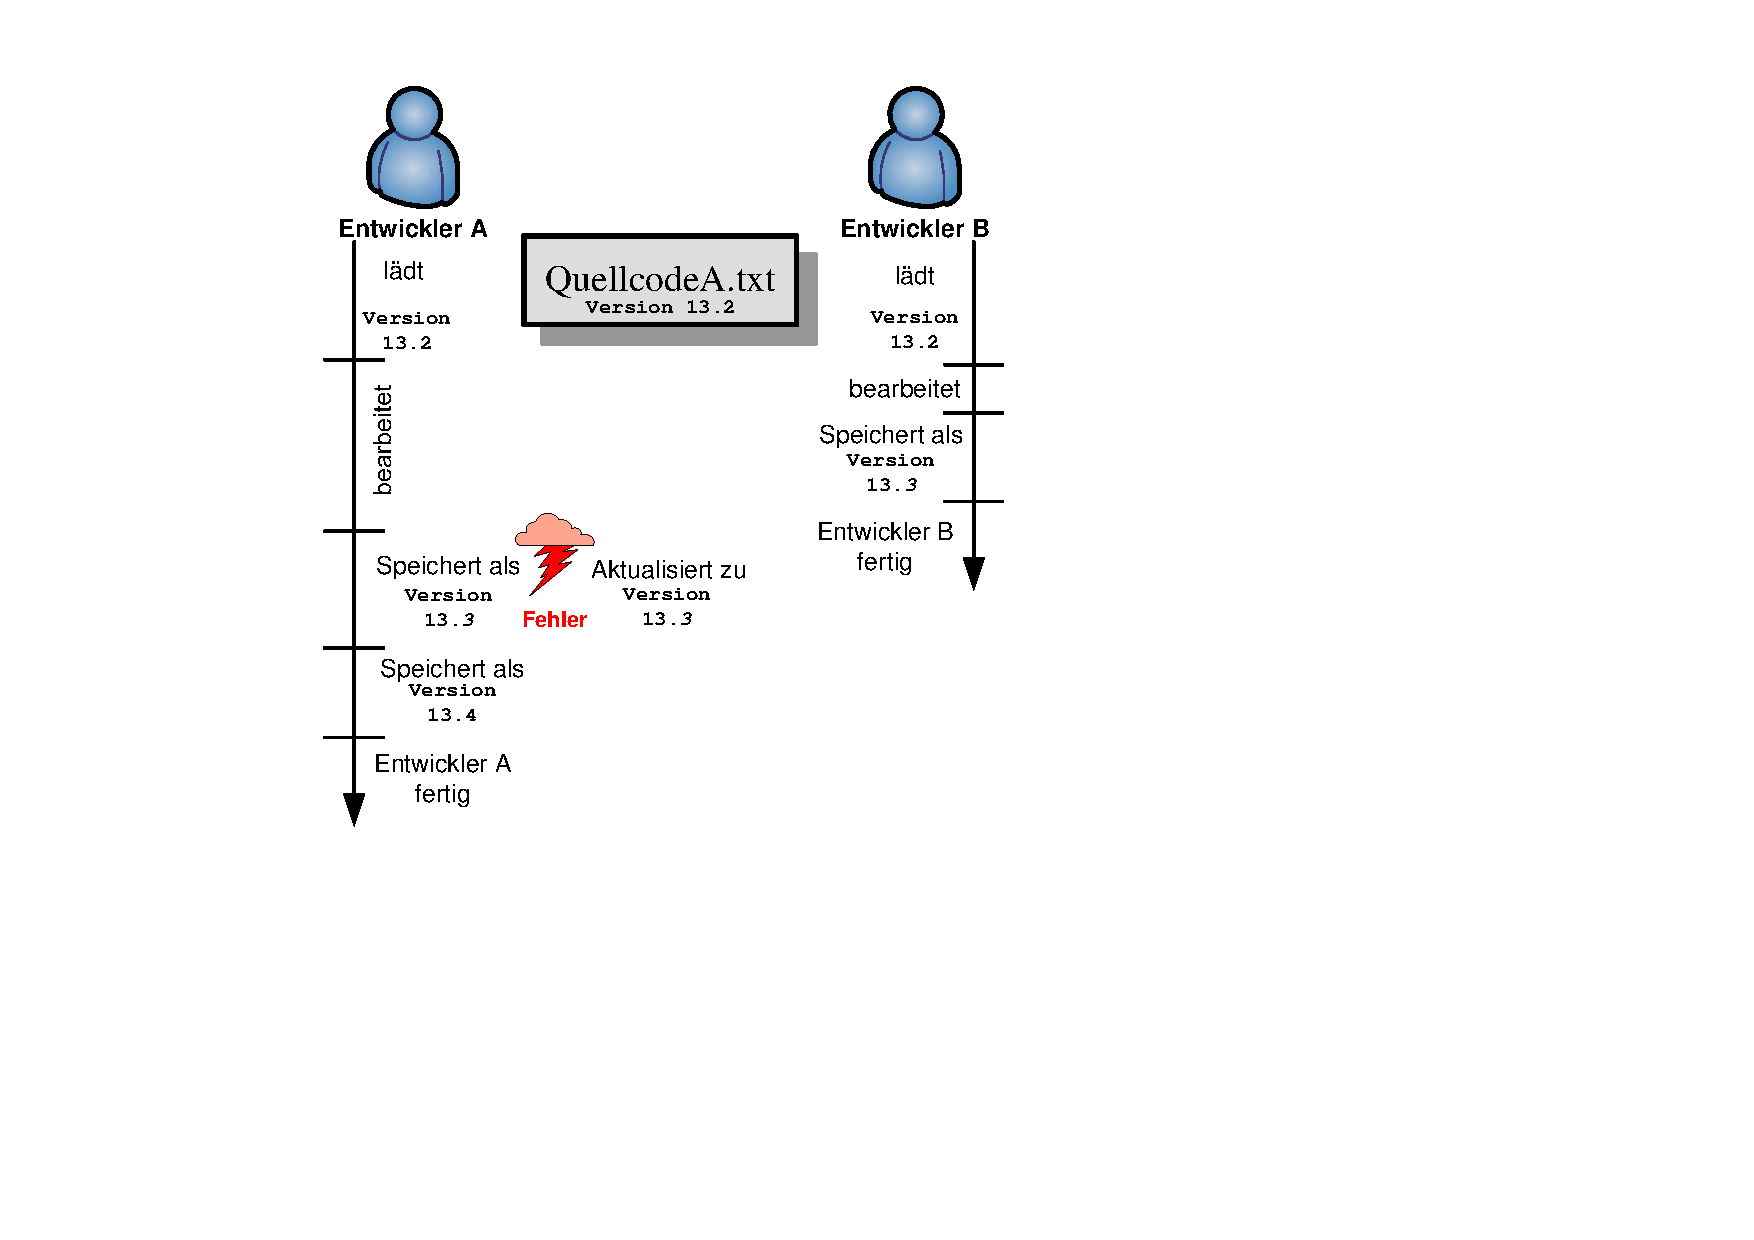
\includegraphics[scale=1.0]{images/kontinuierlicheGenerationsfolge.pdf}
	\caption{Kontinuierliche Entwicklung}
	\label{fig:kontinuerlicheEntwicklung}
\end{figure}
Da im Laufe der Projektzeit viele �nderungen an dem Projekt im Repository gespeichert werden, ist der Speicherplatz enorm. Der Versionsverwaltungsserver speichert jedoch nicht jede Revision komplett in seinem Repository. Die erste Revision einer Datei muss komplett gespeichert werden, f�r alle darauf folgenden Revisionsst�nde werden nur die Unterschiede zur Vorg�ngerversion gespeichert, siehe auch \vref{fig:vvspeicherbedarf}. Der Versionsverwaltungsserver kann aus diesen Informationen jeden Revisionsstand wieder herstellen und bietet somit eine \emph{platzsparende M�glichkeit zur Speicherung} der Revisionen.
\begin{figure}[tbp]
	\centering
	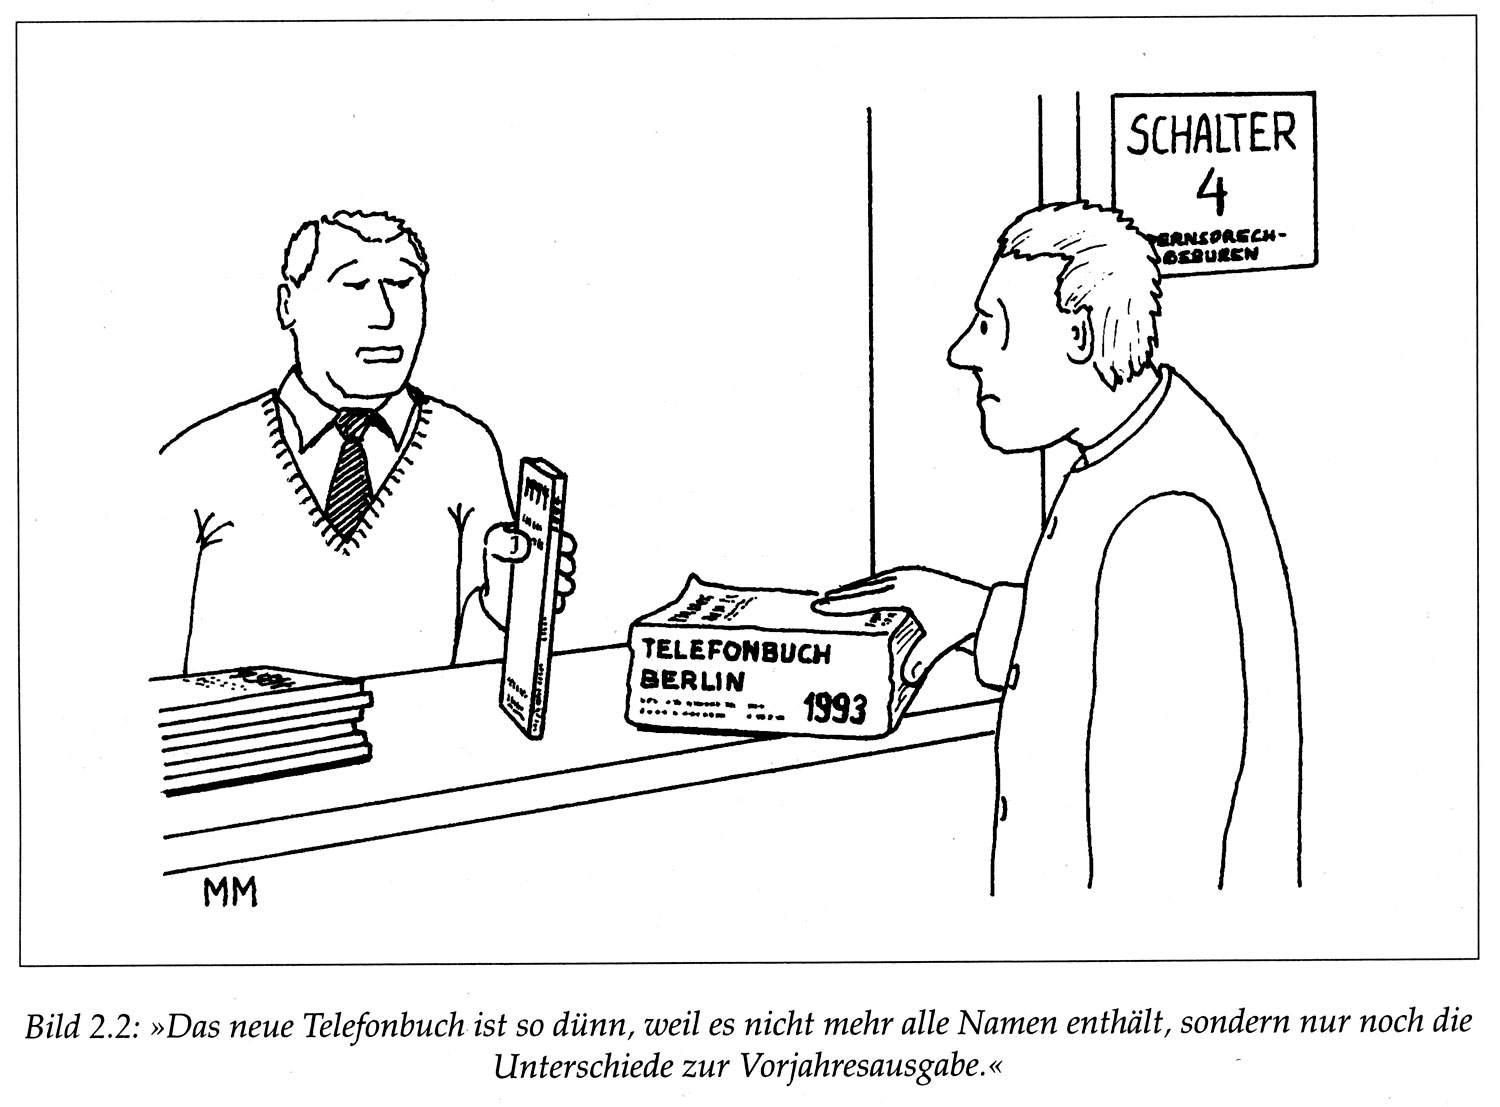
\includegraphics[scale=0.75]{images/vv-speicherbedarf.jpg}
	\caption{Speicherbedarf einer Versionsverwaltung \citep[Bild 2.2]{Herold1995}}
	\label{fig:vvspeicherbedarf}
\end{figure}
Ein Versionsverwaltungsserver bietet �ber verschiedene Sicherheitsmechanismen \emph{Schutz vor unberechtigtem Zugriff}. Dabei muss sich jeder Entwickler �ber einen definierten Mechanismus authentisieren, meist anhand eines Benutzernamens mit einem dazugeh�ren Passwort. Dazu werden abgestufte Zugriffsrechte f�r verschiedene Projektmitglieder auf einzelne Projektteile vergeben, meist anhand der Zust�ndigkeit der Projektmitglieder. Bei der Speicherung eines neues Versionsstandes im Repository wird immer der Benutzer mit gespeichert, damit ist es m�glich, nachzuvollziehen, welcher Benutzer welche �nderungen vorgenommen hat. Ein weitere wichtige Aufgabe einer Versionsverwaltung ist die \emph{Kostenreduzierung}. Durch die bereits erw�hnten Aufgaben einer Versionsverwaltung verringert sich der organisatorische Aufwand des Projektes, Fehler werden vermieden und ein weltweit aktives Team kann gleichzeitig an dem Projekt arbeiten \citep{Fogel2002,Herold1995,Rechenberger1994,Wikipedia2005}. \\
In den folgenden zwei Unterabschnitten werden zwei verschiedene Versionsverwaltungen beschrieben.







%====================================
\subsection{Concurrent Versions System - CVS}






%====================================
\subsection{Subversion - SVN}




\begin{figure}[htbp]
	\centering
	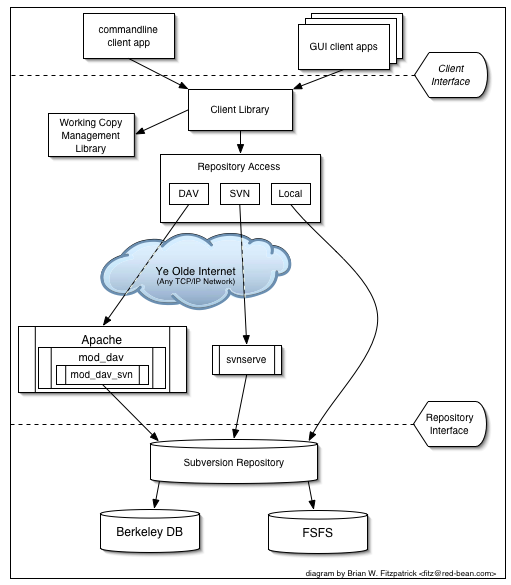
\includegraphics[scale=0.65]{images/subversion-architektur.png}
	\caption{Subversion's Architektur \citep[Kap.~1]{Collins-Sussman2005}}
	\label{fig:svnarchitekur}
\end{figure}

\url{http://better-scm.berlios.de/comparison/comparison.html}





%Hier danach nicht mehr schreiben
\label{sec:tech-Versionsverwaltung-ende}